\chapter{Perturbaciones dependientes del tiempo}
Supongamos que el hamiltoniano tiene dependencia temporal:
\begin{equation}
  \Ham(t) = \Ham_0 + \lambda \Ham_1(t)
\end{equation}
donde $\Ham_0$ es resoluble o al menos dependiente del tiempo. La
evolución temporal de las funciones de onda vendrá dada por la
ecuación de Schrödinger, $\Ham \Psi= i \hbar \dot \Psi$.

Se considera que la perturbación empieza a influir en la
evolución del sistema en un instante $t_0$, modificando los
autoestados iniciales $\varphi_i$ para convertirlos en $\psi(t)$. La
probabilidad de medir uno de los autoestados de $\Ham(t)$ con energía
$E_f$, $\varphi_f$, será:
\begin{equation}
  P_{if}(t)=\abs{\braket{\varphi_f}{\psi(t)}}^2
\end{equation}

Expresamos dicho $\psi(t)$ en función de la base de autoestados de
$\Ham_0$,
\begin{equation}
  \psi(\boldrm{r},t) = \sum_{n} a_n(t) \exp \left( \frac{-i E_n
    }{\hbar} t \right) \varphi_n(\boldrm{r})
\label{eq:psitemp}
\end{equation}
Al coeficiente\marginnote{$a_n(t) = \braket{\varphi_n}{\psi(t=0)}$} dependiente
del tiempo, $a_n(t) e^{\frac{-iE_n}{\hbar}t}$, se le denota por comodidad $b_n(t)$ y es
equivalente a $\braket{\varphi_n}{\psi(t)}$. Si $\lambda=0$ obtenemos que $a(t) =
\text{cte.}$ y se tiene la evolución temporal habitual.

Sustituyendo \eqref{eq:psitemp} en la ecuación de Schrodinger y
simplificando se
obtiene:
\begin{equation}
  \sum_{n} i \hbar \dot{a}_n \varphi_n e^{\frac{-iE_n}{\hbar}t} = \sum_{n}  \lambda a_n \Ham_1 \varphi_n e^{\frac{-iE_n}{\hbar}t} 
\end{equation}
Resolvemos la ecuación vectorial proyectando sobre un vector
$\bra{\varphi_k}$:
\begin{equation}
  i \hbar\dot{a}_k e^{\frac{-iE_k}{\hbar}t} = \sum_{n} \lambda a_n
  e^{\frac{-iE_n}{\hbar}t} \mel{\varphi_k}{\Ham_1}{\varphi_n}
\end{equation}
donde $k\in \mathbb{Z}^+$, por lo que tenemos infinitas ecuaciones
diferenciales acopladas. Hasta aquí no se ha realizado ninguna
aproximación; efectuamos la primera, dada por
\begin{equation}
  a_k = a_k^{(0)} + \lambda a_k^{(1)} + \lambda^2 a_k^{(2)} + \ldots
\end{equation}
Sustituyendo esta aproximación y coleccionando potencias de $\lambda$
obtenemos:
\begin{equation}
  \begin{split}
    \lambda^0:\ \ & \dot{a}_k^{(0)} = 0 \\ 
    \lambda^1:\ \ & \dot{a}_k^{(1)} = \frac{1}{i \hbar} \sum_{n}
    \matrixel{\varphi_k}{\Ham_1}{ \varphi_n} a_k^{(0)} \exp \left(i\omega_{k_n} t \right) \\ 
    \lambda^2: \ \ & \cdots
  \end{split}
\end{equation}
La primera ecuación refleja el caso en que no hay perturbación,
$a^{(0)}=\text{cte.}$ Si bien es posible desarrollar la aproximación a
mayor orden que $1$, nos detendremos aquí.

Nuestras condiciones iniciales son ausencia de perturbación para $t<0$
y $\varphi_i$ conocida como estado inicial. Esto implica para las $a(t)$ que
\begin{equation}
  a_k(0)  = a_k^{(0)}(0) +\lambda a_k^{(1)}(0) + \ldots = \delta_{ki}
\end{equation}
Para $\lambda=0$ obtenemos $a_k^{(0)}(0)=a_k(0)=\delta_{ki}$.

En $a_k^{(1)}$ se obtiene, integrando desde el inicio de la
perturbación ($t=0$) hasta su final ($t=t$):
\begin{equation}
  \begin{split}
    \dot{a}_k^{(1)} &= \frac{1}{i \hbar} \matrixel{\varphi_k}{\Ham_1}{\varphi_i}
    e^{i\omega_{k_i}t}\\
    a_k^{(1)}(t) &= \frac{1}{i \hbar} \int_0^t \matrixel{\varphi_k}{\Ham_1(\tau)}{\varphi_i}
    e^{i\omega_{k_i}\tau} \dd{\tau}
  \end{split}
\end{equation}
donde $a_k^{(1)}(0)=0, \ \forall k$. Obtenemos que $P_{if}(t)$ a
primer orden es
\begin{equation}
  P_{if}(t)= \abs{a_f(t)}^2 = \abs{a_f^{(0)}(t) + \lambda a_f^{(1)}(t)\cdot
    t + \order{t^2}}
\end{equation}
y como $a_f^{(0)}(t)=0$ para $f\neq i$ obtenemos
\begin{equation}
  \boxed{
  P_{if}(t) = \frac{1}{\hbar^2} \abs{ \int_0^t
    \matrixel{\varphi_f}{\Ham_1}{\varphi_i} e^{i \omega_{fi} \tau}\dd{\tau} }^2
}
\end{equation}

\section{Perturbación armónica}
Es la perturbación más frecuente. Tenemos una perturbación $W\cos \omega
t$, con $W$ función de $\boldrm{r}$, $\boldrm{p}$, el espín, ...
 pero no de $t$ ni de sus
derivadas. Calculamos $P_{if}$:
\begin{equation}
  \begin{split}
    P_{if} &= \frac{1}{\hbar^2} \abs{\int_0^t \mel{\varphi_f}{W \cos \omega \tau}{\varphi_i}
      e^{i\omega_{fi}\tau}\dd{\tau}}^2 = \\
    &= \frac{1}{\hbar^2} \abs{W_{fi}
      \int_0^t \cos ( \omega \tau) e^{i\omega_{fi}\tau}\dd{\tau}}^2 = \\
    &= \frac{1}{\hbar^2} \abs{W_{fi}
      \int_0^t \frac{1}{2} \left(
          e^{i\omega\tau}+e^{-i\omega\tau)} \right)
        e^{i\omega_{fi}\tau}\dd{\tau}}^2 = \\
      &= \frac{\abs{W_{fi}}^2}{4 \hbar^2} \abs{ 
        \frac{1- e^{i(\omega_{fi}+\omega)t}}{\omega_{fi}+\omega} 
        +
        \frac{1- e^{i(\omega_{fi}-\omega)t}}{\omega_{fi}-\omega} 
      }^2=  \\
      &= \frac{\abs{W_{fi}}^2}{4 \hbar^2} \abs{ A_+ + A_-}^2
  \end{split}
\end{equation}
Para tener una forma más analizable, utilizamos que
\begin{align}
  A_\pm &= -i e^{i (\omega_{f_i \pm \omega}) t/2} \frac{\sin \left[  
    (\omega_{fi}\pm \omega)\frac{t}{2} 
\right]
}{(\omega_{fi}\pm \omega
          \frac{t}{2})} \\
  \abs{A_\pm} &= 1\cdot \abs{ \frac{\sin \left[  
    (\omega_{fi}\pm \omega)\frac{t}{2} 
\right]
}{(\omega_{fi}\pm \omega
          )\frac{t}{2}} }
\end{align}

Puede verse la forma funcional de $A_\pm$ en la figura \ref{fig:apm}.


\begin{marginfigure}
    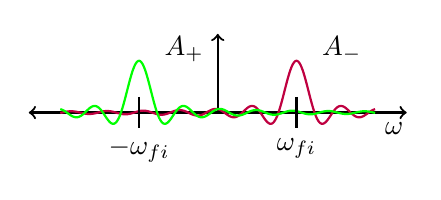
\begin{tikzpicture}[xscale=0.4,yscale=2]
        \draw [thick, <->] (-6,0) -- (6,0);
        \draw [thick, ->] (0,0) -- (0,0.5) ;
        \draw[color=purple, thick, domain=-5:5, samples=300] 
        plot (\x, {0.06*(sin(2*3.1415*50*(\x -2.5))/(\x -2.5)});
        \draw node [right] at (-2,0.4) {$A_+$};
        \draw[color=green, thick, domain=-5:5, samples=300] 
        plot (\x, {0.06*(sin(2*3.1415*50*(\x +2.5))/(\x +2.5)});
        \draw node [right] at (3,0.4) {$A_-$};
        \draw node [below right] at (5,0) {$\omega$};
        \draw [thick] (-2.5,0.1) -- (-2.5,-0.1);
        \draw node [below] at (-2.5,-0.1) {$-\omega_{fi}$};
        \draw [thick] (+2.5,0.1) -- (+2.5,-0.1);
        \draw node [below] at (2.5,-0.1) {$\omega_{fi}$};
    \end{tikzpicture}
    \caption{$A_-$ y $A_+$ pueden considerarse no solapantes si
      $\Delta\omega \ll 2\omega_{fi}$. Vemos que las únicas
      frecuencias con probabilidad no despreciable de absorción son aquellas
      con $\omega\simeq\omega_{fi}$.
    }
    \label{fig:apm}
\end{marginfigure}

Como sólo estamos interesados en $\omega>0$, viendo la forma de
$A_++A-$ podemos aproximar $P_{if}$ como
\begin{equation}
  P_{if} \simeq \frac{\abs{W_{if}}^2}{4 \hbar^2} \abs{A_-}^2
\end{equation}
Esta fórmula sólo será valida cuando $A_-$ y $A_+$ estén bastante
separadas, es decir,
\begin{equation}
  t \gg \frac{2\pi}{\omega_{fi}}
\end{equation}

Esta condición\footnote{Se puede expresar de manera alternativa como
  $\hbar\omega_{fi}t\gg 2\pi \hbar$, es decir \[ \Delta E \Delta t \gg
    h \] Esto es sólo una regla memotécnica, no un principio de incertidumbre. } puede entenderse como que el tiempo que el sistema está
siendo perturbado ha de ser de unos cuantos periodos, para que ``se
entere'' de la perturbación.

Notar que estamos exigiendo $t$ grandes para poder emplear la
aproximación, pero si son demasiado grandes ya no valdría la
aproximación a primer orden que hemos hecho\footnote{Estamos
suponiendo que la función de ondas sólo varía un poco debido a la perturbación.}.

\section{Onda electromagnética}
Consideremos una onda electromagnética del estilo
\begin{align}
  \boldrm{E}(\boldrm{r},t) &= \boldrm{E}_0 \cos
  (\boldrm{k}\boldrm{r}-\omega t) \\
  \boldrm{B}(\boldrm{r},t) &= \frac{\boldrm{E}(\boldrm{r},t)}{c}
\end{align}
Como $\cos(\boldrm{k}\boldrm{r}-\omega t) =
\cos(\boldrm{k}\boldrm{r})\cos(\omega t) -
\sin(\boldrm{k}\boldrm{r})\sin (\omega t)$, podemos suponer
$\boldrm{k}\boldrm{r}$ despreciable\footnote{La suposición es
  equivalente a decir que el tamaño del sistema es mucho menor que la
  longitud de onda. Para una frecuencia visible, como el color amarillo, esto supone que es sistema es
  mucho menor de \SI{600}{\nano\metre}. Siendo que el tamaño atómico
  es del orden del Angstrom, es una buena aproximación.} y aproximar
$\cos(\boldrm{k}\boldrm{r}-\omega t) \simeq
\cos(\boldrm{k}\boldrm{r})$. A esta aproximación se le llama
\emph{aproximación dipolar}. 

Calculamos las energías del campo eléctrico y el magnético:
\begin{align}
  E_E &= e \boldrm{r} \boldrm{E} \sim e a_0 E_0\\
  E_B &= \frac{\mu_{\scriptstyle B}}{\hbar} (\boldrm{L}+g_s
        \boldrm{S}) \boldrm{E} \sim \frac{e \hbar}{2mc} E_0
\end{align}
donde se ha aproximado $\abs{\boldrm{r}}\simeq a_0$ y
$\abs{\boldrm{L}+g_s \boldrm{S}}\simeq \hbar$. Vemos que la energía de
interacción con el campo eléctrico es muy superior a la
magnética\footnote{En concreto, la razón entre $a_0$ y
$\frac{\hbar}{2mc}$ es del orden de $270$.}
, por lo que pasamos a la llamada \emph{aproximación dipolar
  eléctrica} y despreciamos el efecto del campo magnético. 

La perturbación provocada por el campo electromagnético, con todas
estas aproximaciones, se puede escribir como
\begin{equation}
  \Ham_1 = e \boldrm{E}_0
  \cos \omega t  \sum_{i=1}^Z \boldrm{r}_i
\end{equation}
para $Z$ electrones. 
La probabilidad
de las transiciones para $Z=1$ (hidrógeno) será
\begin{equation}
  P_{if}(t,\Delta\omega) = \frac{1}{4 \hbar^2}
  \abs{\mel{\varphi_f}{e \boldrm{r} \boldrm{E}_0 }{\varphi_i}}^2 F(\Delta\omega,t)
\end{equation}
donde $F(\Delta\omega,t)$ engloba los términos derivados del
$\cos(\omega t)$.
Si definimos como perturbaciones aceptables aquellas que son un orden
de magnitud menor que la energía típica (\SI{0.1}{\eV}) encontramos
que el campo eléctrico ha de ser menor de \SI{1e8}{\volt\per\metre}.
Estos valores se alcanzan sólo en situaciones extremas como la
superficie solar, por lo que la aproximación es buena.

\subsection{Emisión espontánea}
Consideremos un campo electromagnético no monocromático con un vector
de Pointing
\begin{equation}
  \abs{\ev{\boldrm{S}}} = \frac{\varepsilon_0c}{2} E_0^2 = I(\omega)
\end{equation}
donde $\boldrm{E}_0 = E_0 \hat{n}$ y $[I] =
\SI{}{\joule\per\square\metre\per\second}$. La probabilidad de transición
vendrá dada por
\begin{equation}
  P_{if} = \frac{e^2}{2\varepsilon_0 c \hbar^2}
  \abs{\mel{\varphi_f}{\boldrm{r}\hat{n}}{\varphi_i}}^2 \int_0^\infty
  \dd{\omega} I(\omega) F(\omega_{fi}-\omega,t)
\end{equation}
donde
$I(\omega)=I(\omega_{fi})+I'(\omega)(\omega-\omega_{fi})+\cdots$. tras
resolver la
integral\footnote{
En primer lugar, integramos en $\mathbb{R}$ en lugar de en
$\mathbb{R}^+$. Para resolverla, sustituimos
\begin{equation*}
  \begin{cases}
    x &= \frac{1}{2} (\omega_{fi}-\omega) t\\
    \dd{x} &= - \dd{\omega} \frac{t}{2}
  \end{cases}
\end{equation*}
y utilizamos que $F= \text{sinc}^2[\frac{t}{2}(\omega_{fi}-\omega)]$ y
que $\int_\mathbb{R} \frac{\sin^2 x}{x} \dd{x} = \pi$.
} obtenemos:
\begin{equation}
  \begin{split}
    P_{if} &= \frac{e^2\pi}{\varepsilon_0 c \hbar^2}
    \abs{\mel{\varphi_f}{\boldrm{r}\hat{n}}{\varphi_i}}^2 I(\omega_{fi}) \cdot t\\
     &= \frac{4\pi^2\alpha}{\hbar}
    \abs{\mel{\varphi_f}{\boldrm{r}\hat{n}}{\varphi_i}}^2 I(\omega_{fi})\cdot t
  \end{split}
\end{equation}
La variación de estas probabilidades será
\begin{equation}
  \dv{P_{if}}{t} =  \lambda_{if} =
  \frac{4\pi^2\alpha}{\hbar}
  \abs{\mel{\varphi_f}{\boldrm{r}\hat{n}}{\varphi_f}}^2 I(\omega_{fi}) = \text{cte.}
\end{equation}

\marginnote{Notar que como todas las integrales realizadas hasta el
  momento son invariantes ante un intercambio del estado inicial por
  el final la probabilidad de absorción es idéntica a la de emisión, $P_{if}=P_{fi}$.}

Podemos escribir con esta expresión la variación de elecrones en dos
niveles (figura \ref{fig:twolevel}), utilizando $B I(\omega_{fi})=\lambda_{if}$:

\begin{marginfigure}
  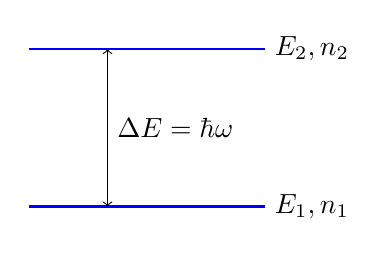
\begin{tikzpicture}[xscale=1,yscale=1]
    \draw [blue,thick, -] (0,0) -- (3,0);
    \draw [blue,thick, -] (0,2) -- (3,2);
    \draw [thin, <->] (1,0) -- (1,2);
    \draw node [right] at (1,1) {$\Delta E = \hbar\omega$};
    \draw node [right] at (3,0) {$E_1,n_1$};
    \draw node [right] at (3,2) {$E_2,n_2$};
  \end{tikzpicture}
  \caption{Sistema de dos niveles}
  \label{fig:twolevel}
\end{marginfigure}

\begin{equation}
  \begin{split}
    \dv{n_2}{t} &= B I(\omega) n_1 - B I(\omega) n_2 \\
    \dv{n_1}{t} &= B I(\omega) n_2 - B I(\omega) n_1 \\
  \end{split}
\end{equation}

Se presupone equilibrio térmico,
\begin{equation}
  \frac{n_2}{n_1} = e^{-\beta\hbar\omega}
\end{equation}

Pero en el equilibrio ambas derivadas son nulas, por lo que $n_2 = n_1
\neq n_1 e^{-\beta \hbar\omega}$. Por tanto, ha de exisitir un término
de emisión espontánea con coeficiente $A$:
\begin{equation}
  \begin{cases}
    \dv{n_2}{t} &= B I(\omega) n_1 - B I(\omega) n_2 - An_2 \\
    \dv{n_1}{t} &= B I(\omega) n_2 - B I(\omega) n_1 + An_2\\
  \end{cases}
\end{equation}

En condiciones de equilibrio obtenemos $B I(\omega) n_1 = [A+B
I(\omega)] n_2$, despejando\footnote{Hay que sustituir
  $\nicefrac{n_2}{n_1}=\exp(-\beta \hbar\omega)$ y $I = c\rho(\omega)=
  \frac{1}{\pi^2c^2}\frac{\hbar\omega^3}{e^{\beta \hbar\omega}}$} $A$ obtenemos:
\begin{equation}
  A = \frac{\hbar\omega^3}{\pi^2c^2}B 
\end{equation}
donde $B\sim \abs{\mel{\varphi_f}{\boldrm{r}\hat{n}}{\varphi_i}}^2$. Hemos
obtenido $A$ con un argumento semiclásico (equilibrio térmico), sin
recurrir a la cuantificación del campo electromagnético.

%%% Local Variables:
%%% mode: latex
%%% TeX-master: "../resumen"
%%% End:
